
\begin{figure}[ht]
\centering

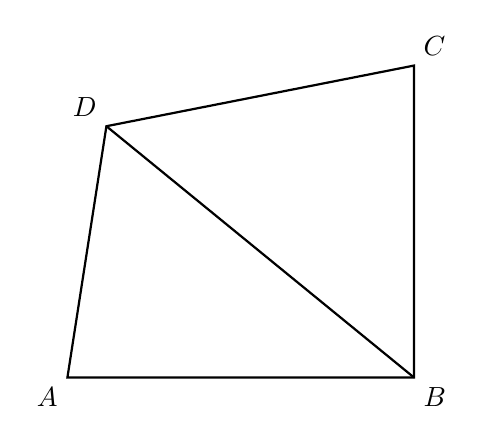
\begin{tikzpicture}[scale=1.1]

    % Vertices
    \coordinate (A) at (0,0);
    \coordinate (B) at (4,0);
    \coordinate (C) at (4,3.6);
    \coordinate (D) at (0.45,2.9);

    % Draw quadrilateral ABCD
    \draw[black, line width=0.8pt]
        (A) -- (D) -- (C) -- (B) -- cycle;

    % Draw diagonal BD
    \draw[black, line width=0.8pt]
        (D) -- (B);

    % Label vertices
    \node[below left] at (A) {$A$};
    \node[below right] at (B) {$B$};
    \node[above right] at (C) {$C$};
    \node[above left] at (D) {$D$};

\end{tikzpicture}

\end{figure}
